\documentclass[class=article, crop=false, 12pt,a4paper]{standalone}
\usepackage{enumitem}
\usepackage{multicol}
\usepackage{etoolbox}
\AtBeginEnvironment{quote}{\singlespacing\small}
\usepackage{setspace}
\onehalfspacing
\usepackage{graphicx}
\usepackage{float}
\usepackage{amsmath}
\usepackage{amssymb}
\usepackage{mathtools}
\usepackage{siunitx}
\sisetup{detect-all}
\begin{document}
\title{Energy balance lab report}
\author{Hasha Dar}
\date{February 4, 2020}
\maketitle
\tableofcontents
\section{Lab data}
\subsection{1 bar}
\begin{multicols}{2}
  \begin{itemize}[noitemsep]
    \item \(T_0\) = 25 degrees
    \item \(T_1\) = 23 degrees
    \item \(P_0\) = 1 \si{bar}
    \item \(P_1\) = 0.05 \si{bar}
    \item \(P_2\) = 1 \si{\bar}
    \item \(V_{in}\) = 285 \si{\liter\per\minute}
    \item \(N\) = 1430 rev\si{\per\second}
    \item \(F\) = 1.5g \si{\newton} FIX THIS
    \item \(\dot{W}_{el}\) = 1150 \si{\watt}
  \end{itemize}
\end{multicols}
\subsubsection{\(T_2\) readings} 
\begin{table}
  \centering
    \begin{tabular}{|c|c|}
      \hline
      Time (\si{\minute}) & \(T_2\) (degrees C)\\
      \hline
      0 & 95\\
      1 & 98\\
      2 & 101\\
      3 & 104\\
      4 & 106\\
      5 & 108\\
      6 & 110\\
      7 & 112\\
      8 & 114\\
      9 & 116\\
      10 & 118\\
      11 & 119\\
      12 & 121\\
      13 & 122\\
      14 & 124\\
      15 & 125\\
      16 & 127\\
      17 & 128\\
      18 & 130\\
      19 & 131\\
      20 & 131\\
      \hline
    \end{tabular}
  \caption{\(T_2\) readings from apparatus with 1 bar compressor}
  \label{table:1}
\end{table}
\subsection{0.6 bar}
\begin{multicols}{2}
  \begin{itemize}[noitemsep]
    \item \(T_0\) = 25 degrees
    \item \(T_1\) = 24 degrees
    \item \(P_0\) = 1 \si{\bar}
    \item \(P_1\) = 0.06 \si{\bar}
    \item \(P_2\) = 1 \si{\bar}
    \item \(V_{in}\) = 310 \si{\liter\per\minute}
    \item \(N\) = 1445 rev\si{\per\second}
    \item \(F\) = 1.5 \si{\kilogram} FIX THIS
    \item \(\dot{W}_{el}\) = 1000 \si{watt}
  \end{itemize}
\end{multicols}
\subsubsection{\(T_2\) readings}
\begin{table}
  \centering
    \begin{tabular}{|c|c|}
      \hline
      Time (\si{\minute}) & \(T_2\) (degrees C)\\
      \hline  
      0 & 63\\
      1 & 68\\
      2 & 71\\
      3 & 74\\
      4 & 77\\
      5 & 79\\
      6 & 81\\
      7 & 84\\
      8 & 86\\
      9 & 88\\
      10 & 89\\
      11 & 91\\
      12 & 92\\
      13 & 94\\
      14 & 95\\
      15 & 97\\
      16 & 98\\
      17 & 99\\
      18 & 101\\
      19 & 102\\
      20 & 103\\
      \hline
    \end{tabular}
  \caption{\(T_2\) readings from apparatus with 0.6 bar compressor}
  \label{table:2}
\end{table}
\subsection{0.3 bar}
\begin{multicols}{2}
  \begin{itemize}[noitemsep]
    \item \(T_0\) = 25 degrees
    \item \(T_1\) = 25 degrees
    \item \(P_0\) = 1 \si{\bar}
    \item \(P_1\) = 0.08 \si{\bar}
    \item \(P_2\) = 1 \si{\bar}
    \item \(V_{in}\) = 320 \si{\liter\per\minute}
    \item \(N\) = 1459 rev\si{\per\second}
    \item \(F\) = 1.5 \si{\kilogram} FIX THIS
    \item \(\dot{W}_{el}\) = 850 \si{watt}
  \end{itemize}
\end{multicols}
\subsubsection{\(T_2\) readings}
\begin{table}
  \centering
    \begin{tabular}{|c|c|}
      \hline
      Time (\si{\minute}) & \(T_2\) (degrees C)\\
      \hline  
      0 & 52\\
      1 & 55\\
      2 & 58\\
      3 & 60\\
      4 & 62\\
      5 & 63\\
      6 & 65\\
      7 & 67\\
      8 & 68\\
      9 & 69\\
      10 & 70\\
      11 & 71\\
      12 & 72\\
      13 & 73\\
      14 & 74\\
      15 & 75\\
      16 & 76\\
      17 & 76\\
      18 & 77\\
      19 & 78\\
      20 & 78\\
      \hline
    \end{tabular}
  \caption{\(T_2\) readings from apparatus with 0.3 bar compressor}
  \label{table:3}
\end{table}
\section{Experiment 1 calculations}
All the calculations completed below were done with data from the 1 bar experiment.
\subsection{Volumetric flow rate}
The formula for the volumetric flow rate is:
\begin{equation}
  \dot{V} = \frac{V_in}{60 \times 10^3} \ \si{\meter\cubed\per\second}
  \label{volflowrate}
\end{equation}
Thus, our volumetric flow rate (using equation (1)) is:
\[ \dot{V} = \frac{285}{60\times 10^3} = \frac{19}{4000} = 4.75 \times 10^{-3} \ \si{\meter\cubed\per\second} \ (3\textrm{sf})\]
\subsection{Mass flow rate}
The specific volume through flowmeter is given by the following equation
\begin{equation}
  v_0 = \frac{RT_0}{P_0} \ (\si{\meter\cubed\per\kg}) \textrm{ where \(R = 0.287 \ \si{\kilo\joule\per\kg\per\kelvin}\)}
  \label{specvol}
\end{equation}
The mass flow rate is given by the following equation:
\begin{equation}
  \dot{m} = \frac{\dot{V}}{v_0} \ \si{\kg\per\second}
  \label{massflowrate}
\end{equation}
Calculating the specific volume (2) and inputting the volume flow rate calculated previously (from equation (1)) our mass flow rate is:
\[ v_0 = \frac{0.287 \cdot (25+273.15)}{100} = 0.856 \ \si{\kg\per\second} \ (3\textrm{sf})  \]
\[ \dot{m} = \frac{4.75 \times 10^{-3}}{0.856} = 5.55 \times 10^{-3} \ \si{\kg\per\second} \ (3\textrm{sf}) \]
\subsection{Energy added to air by compressor}
The equation to calculate the energy added to air by compressor is:
\begin{equation}
  \dot{H}_c = \dot{m}c_P(T_2-T_1) \ (\si{\watt}) \textrm{ where \(c_P\) is 1005 \si{\kilo\joule\kg\per\kelvin}}
  \label{energyaddaircompressor}
\end{equation}
Inputting the variables into equation (4), we get: 
\[ \dot{H}_c = 5.55 \times 10^{-3} \times 1005 \times (131-23) = 602.296 \ \si{\watt} \ (3\textrm{dp}) \]
\subsection{Power out of motor}
The equation for the power out of the motor is:
\begin{equation}
  \dot{W}_{m} = \frac{19.62NFL\pi}{60} \ \si{\watt}
  \label{motorpower}
\end{equation}
Thus, our motor power is:
\[ \dot{W}_{m} = \frac{19.62 \times 1430 \times 1.5 \times 0.2 \times \pi}{60} = 440.712 \ \si{\watt} \ (3\textrm{dp}) \]
\subsection{Heat losses in the compressor}
The equation for the heat emitted from the compressor is:
\begin{equation}
  \dot{Q}_c = \dot{W}_m - \dot{H}_c
  \label{heatlosscompressor}
\end{equation}
Thus, our motor heat losses are:
\[ \dot{Q}_c = 440.712 - 602.296 = -161.685 \ \si{\watt} \ (3\textrm{dp}) \]
\section{Experiment 1 discussion}
\subsection{Plot graph of outlet temperature against time}
Importing the data into MATLAB, I plotted the data on a graph.
\begin{figure}
  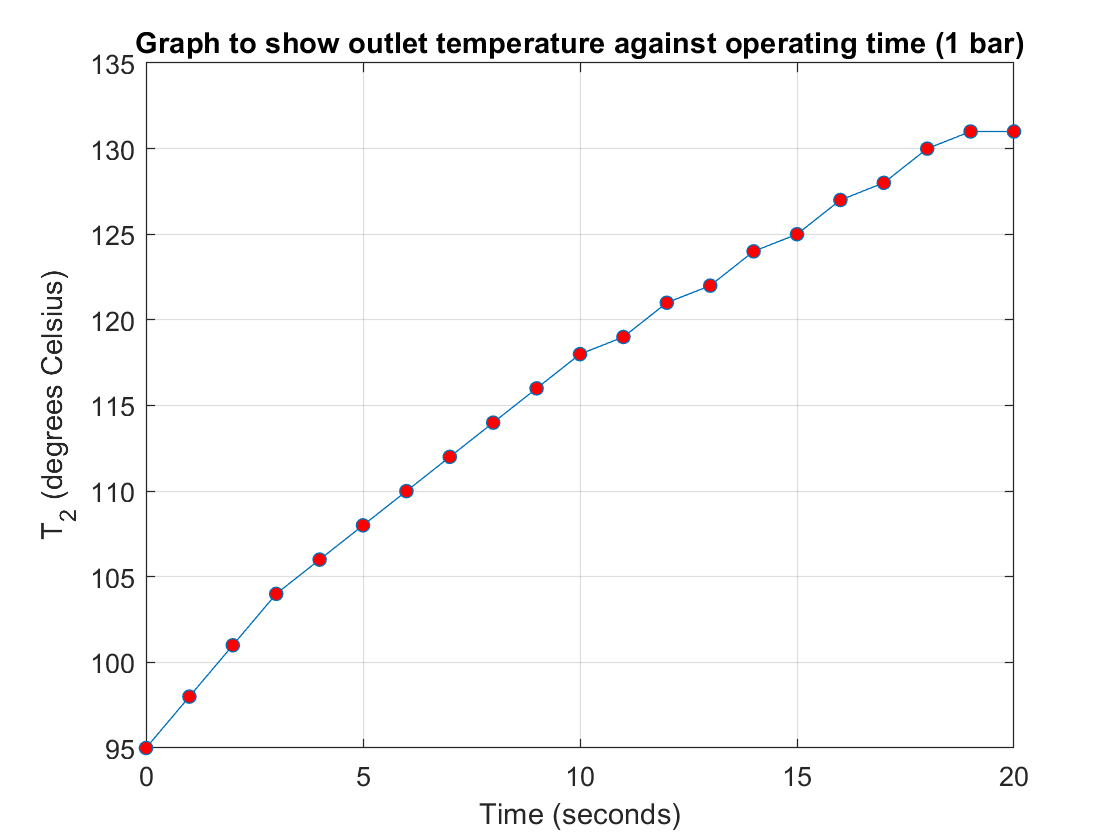
\includegraphics[width = 0.9 \textwidth]{./img/T21vsTimeGraph}
  \caption{Plot of \(T_2\) against the operating time of the apparatus (1 bar)}
  \label{ref:T21vsTime1bar}
\end{figure}
\begin{figure}
  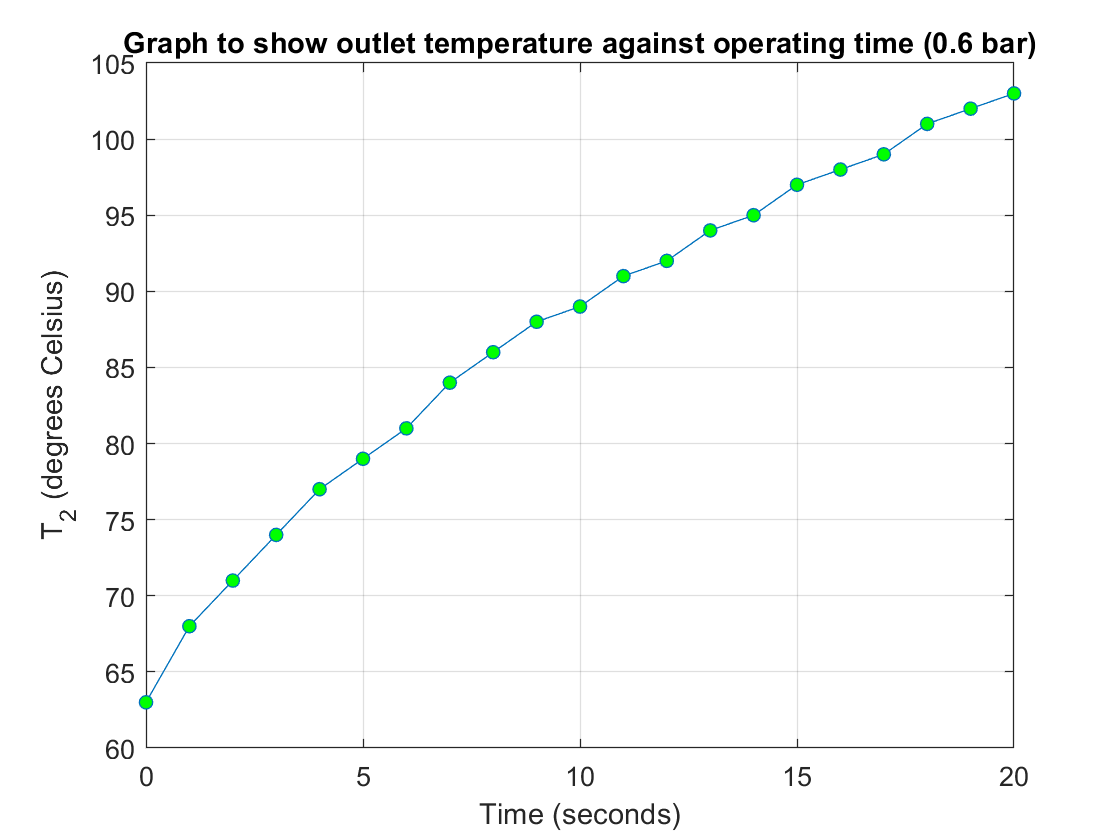
\includegraphics[width = 0.9 \textwidth]{./img/T206vsTimeGraph}
  \caption{Plot of \(T_2\) against the operating time of the apparatus (0.6 bar)}
  \label{ref:T206vsTime1bar}
\end{figure}
\begin{figure}
  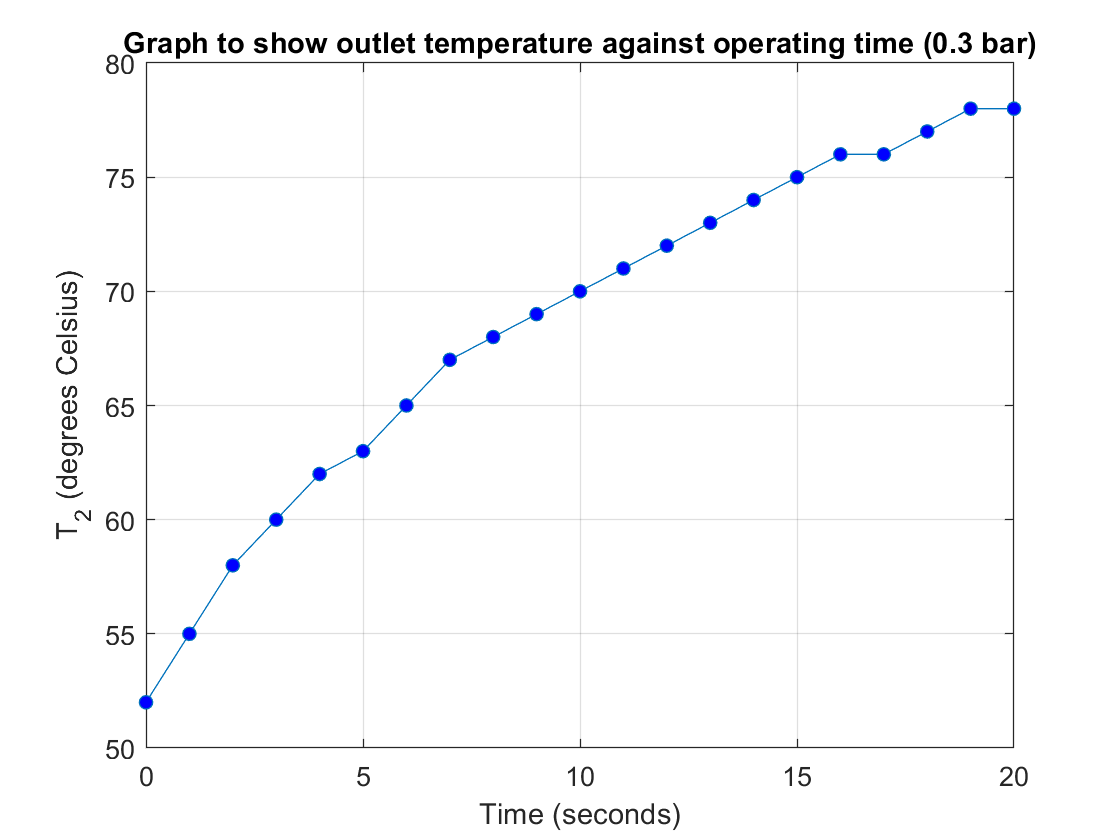
\includegraphics[width = 0.9 \textwidth]{./img/T203vsTimeGraph}
  \caption{Plot of \(T_2\) against the operating time of the apparatus (0.3 bar)}
  \label{ref:T203vsTime1bar}
\end{figure}
NOT IN SECONDS FIX
\subsubsection{Why does the graph have this shape?}

\section{Experiment 2 calculations}
\subsection{Specific volume of air at atmosphere and the inlet and outlet of compressor}
We can calculate the specific volumes at atmosphere, before and after the compressor using equation (\ref{specvol}), which is shown below.
\begin{equation}
  v_0 = \frac{RT_0}{P_0} \ (\si{\meter\cubed\per\kg}) \textrm{ where \(R = 0.287 \ \si{\kilo\joule\per\kg\per\kelvin}\)}
  \tag{\ref{specvol}}
\end{equation}
Thus, at atmosphere our specific volume of air is:
\[ v_0 = \frac{0.287 \times (25+273.15)}{100} = 0.856 \ \si{\meter\cubed\per\kg} \ (3\textrm{sf}) \]
The temperature is constant before the compressor and \(T_2\) approaches a constant value after some time, hence we can use a formula for specific volume where T is constant:
\begin{equation}
  v_1 = v_0 \times \left( \frac{P_0}{P_0 - P_1} \right) \ \si{\meter\cubed\per\kg}
  \label{constpspecvol}
\end{equation}
Using equation (\ref{constpspecvol}), the specific volume before the compressor is:
\[ v_1 = 0.856 \times \left( \frac{100}{100-5} \right) = \frac{428}{475} = 0.901 \ \si{\meter\cubed\per\kg} \ (3\textrm{sf}) \textrm{ (1 bar)} \]
\[ v_1 = 0.856 \times \left( \frac{100}{100-6} \right) = \frac{214}{235} = 0.911 \ \si{\meter\cubed\per\kg} \ (3\textrm{sf}) \textrm{ (0.6 bar)} \]
\[ v_1 = 0.856 \times \left( \frac{100}{100-8} \right) = \frac{107}{115} = 0.930 \ \si{\meter\cubed\per\kg} \ (3\textrm{sf}) \textrm{ (0.3 bar)} \]
Using equation (\ref{constpspecvol}), the specific volume after the compressor is:
\[ v_2 = 0.856 \times \left( \frac{100}{100+100} \right) = \frac{107}{115} = 0.428 \ \si{\meter\cubed\per\kg} \ (3\textrm{sf}) \textrm{ (1, 0.6, 0.3 bar)} \]
\subsection{Volumetric flow rate of air}
Using equation (\ref{volflowrate}) we can calculate the volumetric flow rate of air.
\begin{equation}
  \dot{V} = \frac{V_in}{60 \times 10^3} \ \si{\meter\cubed\per\second}
  \tag{\ref{volflowrate}}
\end{equation}
\[ \dot{V} = \frac{285}{60\times 10^3} = \frac{19}{4000} = 4.75 \times 10^{-3} \ \si{\meter\cubed\per\second} \ (3\textrm{sf}) \ \textrm{ (1 bar)}\]
\[ \dot{V} = \frac{310}{60\times 10^3} = \frac{31}{6000} = 5.17 \times 10^{-3} \ \si{\meter\cubed\per\second} \ (3\textrm{sf}) \ \textrm{ (0.6 bar)}\]
\[ \dot{V} = \frac{320}{60\times 10^3} = \frac{2}{375} = 5.33 \times 10^{-3} \ \si{\meter\cubed\per\second} \ (3\textrm{sf}) \ \textrm{ (0.3 bar)}\]
\subsection{Mass flow rate of air}
The mass flow rate of air can be calculated using equation (\ref{massflowrate})
\begin{equation}
  \dot{m} = \frac{\dot{V}}{v_0} \ \si{\kg\per\second}
  \tag{\ref{massflowrate}}
\end{equation}
Calculating the specific volume and inputting the volume flow rate calculated previously (from equation (1)) our mass flow rate is:
\[ v_0 = \frac{0.287 \cdot (25+273.15)}{100} = 0.856 \ \si{\kg\per\second} \ (3\textrm{sf})  \]
\[ \dot{m} = \frac{4.75 \times 10^{-3}}{0.856} = 5.55 \times 10^{-3} \ \si{\kg\per\second} \ (3\textrm{sf}) \textrm{ (1 bar)} \]
\[ \dot{m} = \frac{5.17 \times 10^{-3}}{0.856} = 6.04 \times 10^{-3} \ \si{\kg\per\second} \ (3\textrm{sf}) \textrm{ (0.6 bar)} \]
\[ \dot{m} = \frac{5.33 \times 10^{-3}}{0.856} = 6.23 \times 10^{-3} \ \si{\kg\per\second} \ (3\textrm{sf}) \textrm{ (0.3 bar)} \]
\subsection{Theoretical mass flow rate of air}
The compressors swept volume is \(V_{comp} = 2.67 \times 10^{-4}\), hence we can calculate the theoretical mass flow rate using equation (\ref{massflowrate})
\begin{equation}
  \dot{m} = \frac{\dot{V}_{comp} \times N}{60 \times v_0} \ \si{\kg\per\second}
  \tag{\ref{massflowrate}}
\end{equation}
\[ \dot{m} = \frac{2.67 \times 10^{-4} \times 1430}{60 \times 0.856} = 7.43 \times 10^{-3} \ \si{\kg\per\second} \ (3\textrm{sf}) \textrm{ (1 bar)}\]
\[ \dot{m} = \frac{2.67 \times 10^{-4} \times 1445}{60 \times 0.856} = 7.51 \times 10^{-3} \ \si{\kg\per\second} \ (3\textrm{sf}) \textrm{ (0.6 bar)}\]
\[ \dot{m} = \frac{2.67 \times 10^{-4} \times 1459}{60 \times 0.856} = 7.58 \times 10^{-3} \ \si{\kg\per\second} \ (3\textrm{sf}) \textrm{ (0.3 bar)}\]

\listoffigures
\end{document}